\section{System architecture}

The developed 3D/4D GIS system has a two-tier architecture (Figure \ref{fig:sys_arch_2tier}). The {\em server} contains the master copy of the data and a PostgreSQL database called \textit{viaappiadb}. The {\em clients} download or request the data required for visualization and run the 3D/4D viewer locally or via a Web application which connects to the remote database when required.
 
A diagram of the data preparation framework which is executed in the server is shown in Figure \ref{fig:sys_arch_data_framework}. The raw data is converted to the OpenSceneGraph (http://www.openscenegraph.org) binary format. The \textit{viaappiadb} database is filled with meta-data information of the location of the raw data and the converted data. The archaeological information with attribute data for the several sites is provided in a Microsoft Access file. It needs to be converted to the PostgreSQL format before being imported into the main database. The footprints are provided in a PostgreSQL dump file and are imported into the \textit{viaappiadb} database as well.

\begin{figure}[!ht]
 \centering
 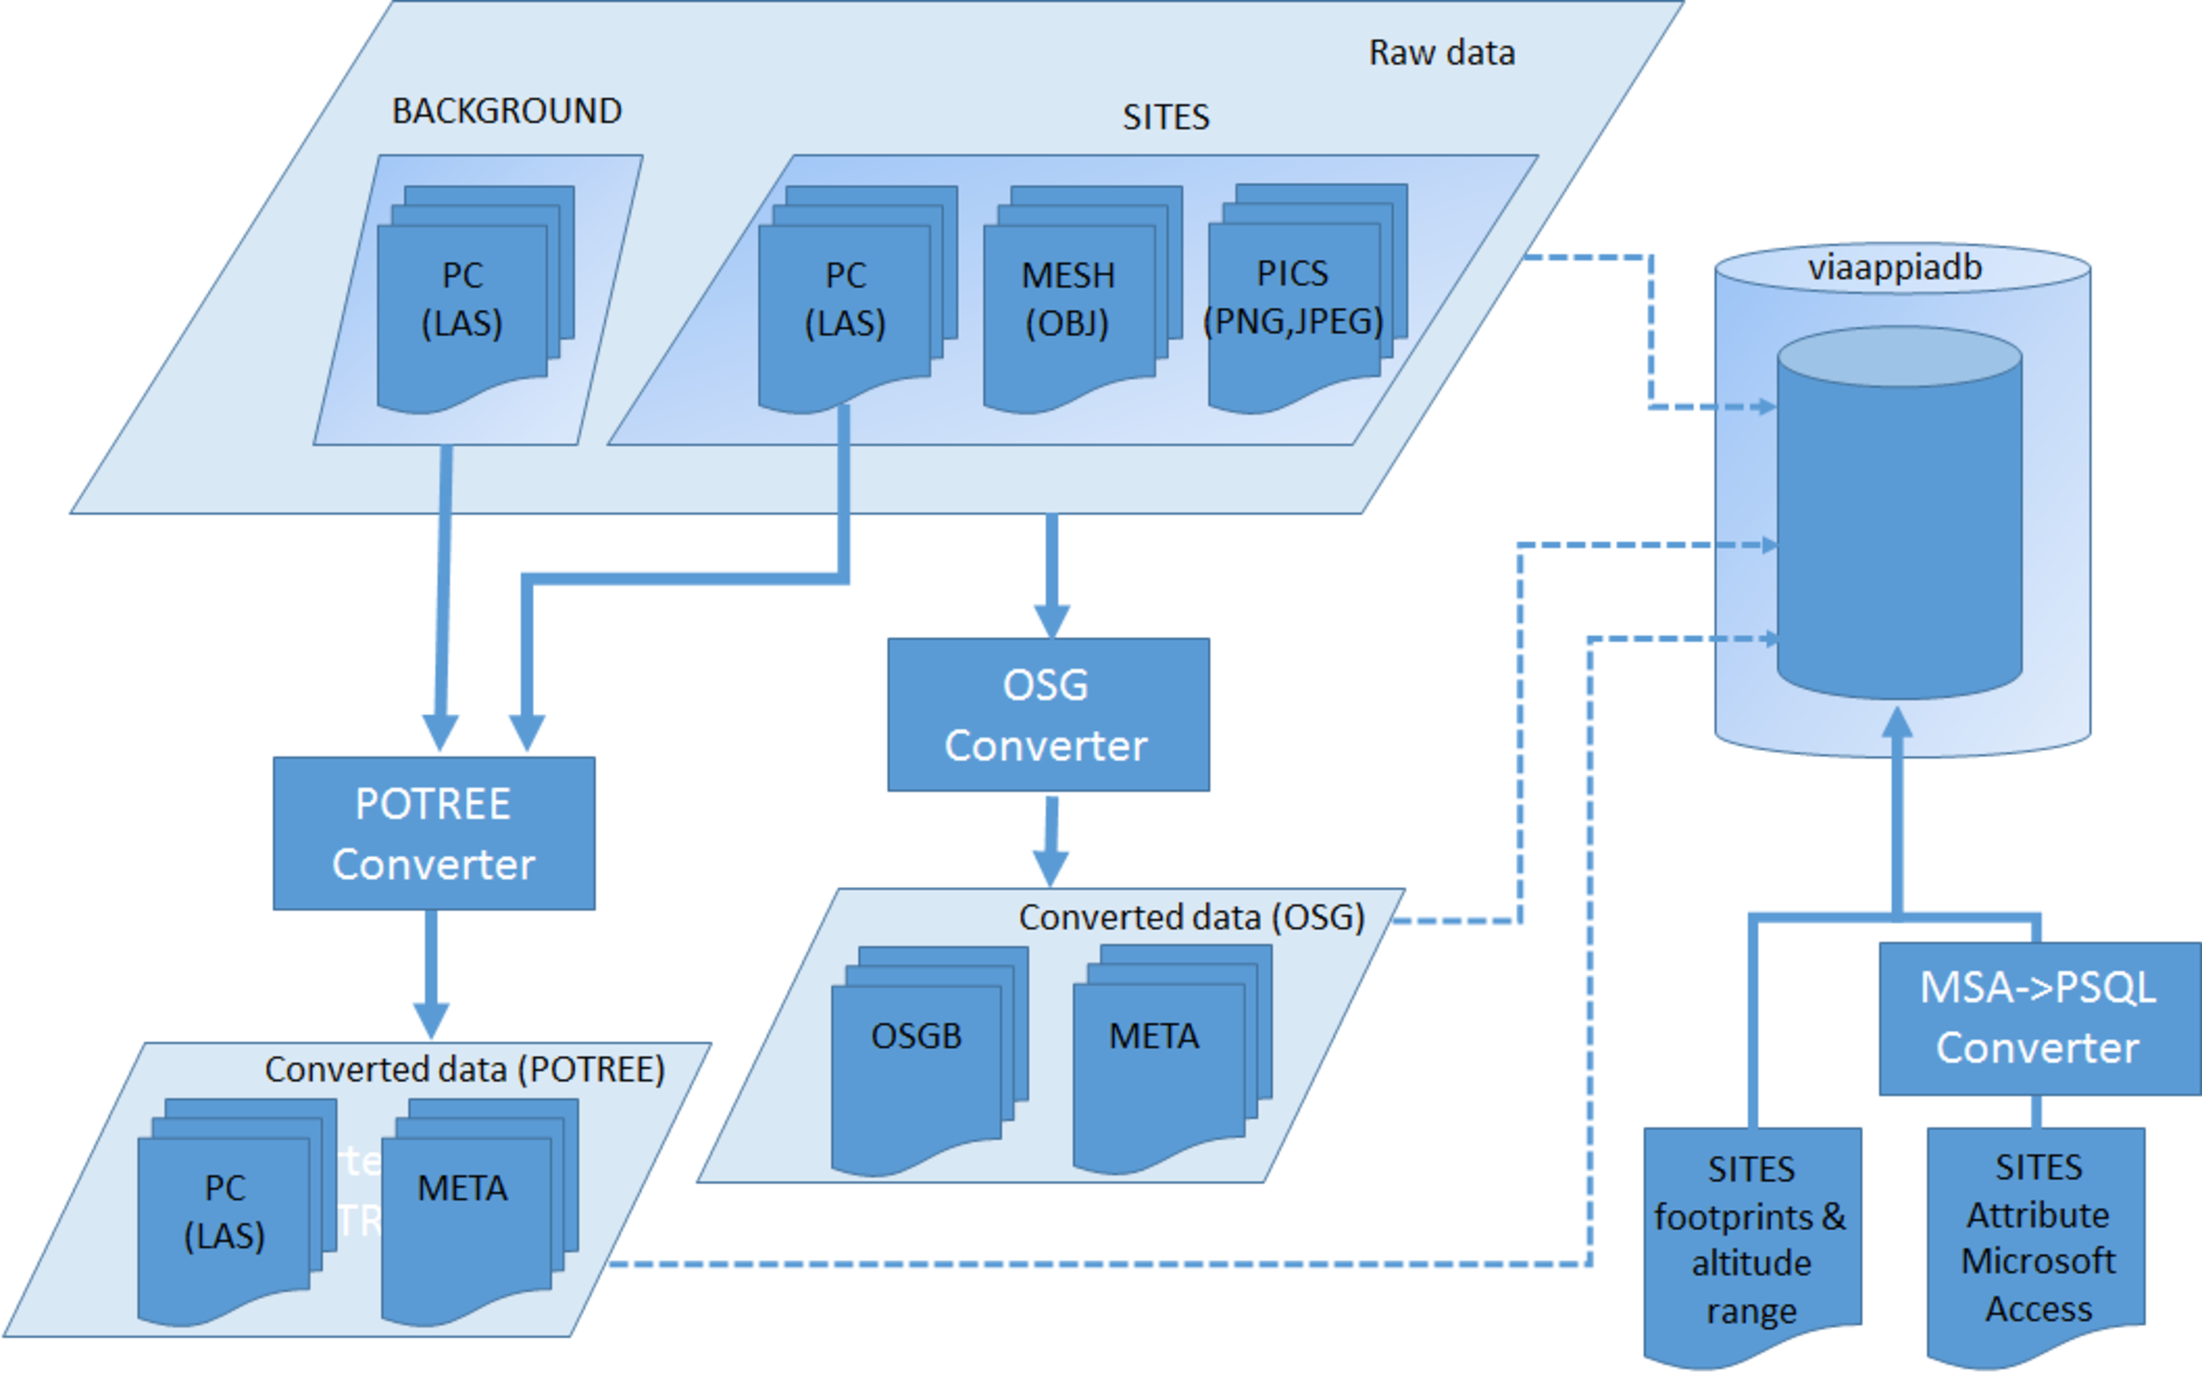
\includegraphics[width=0.4\textwidth]{fig/system_architecture/DataFramework.pdf}
 \caption{}
 \label{fig:sys_arch_data_framework}
\end{figure}

\begin{figure}[!ht]
 \centering
 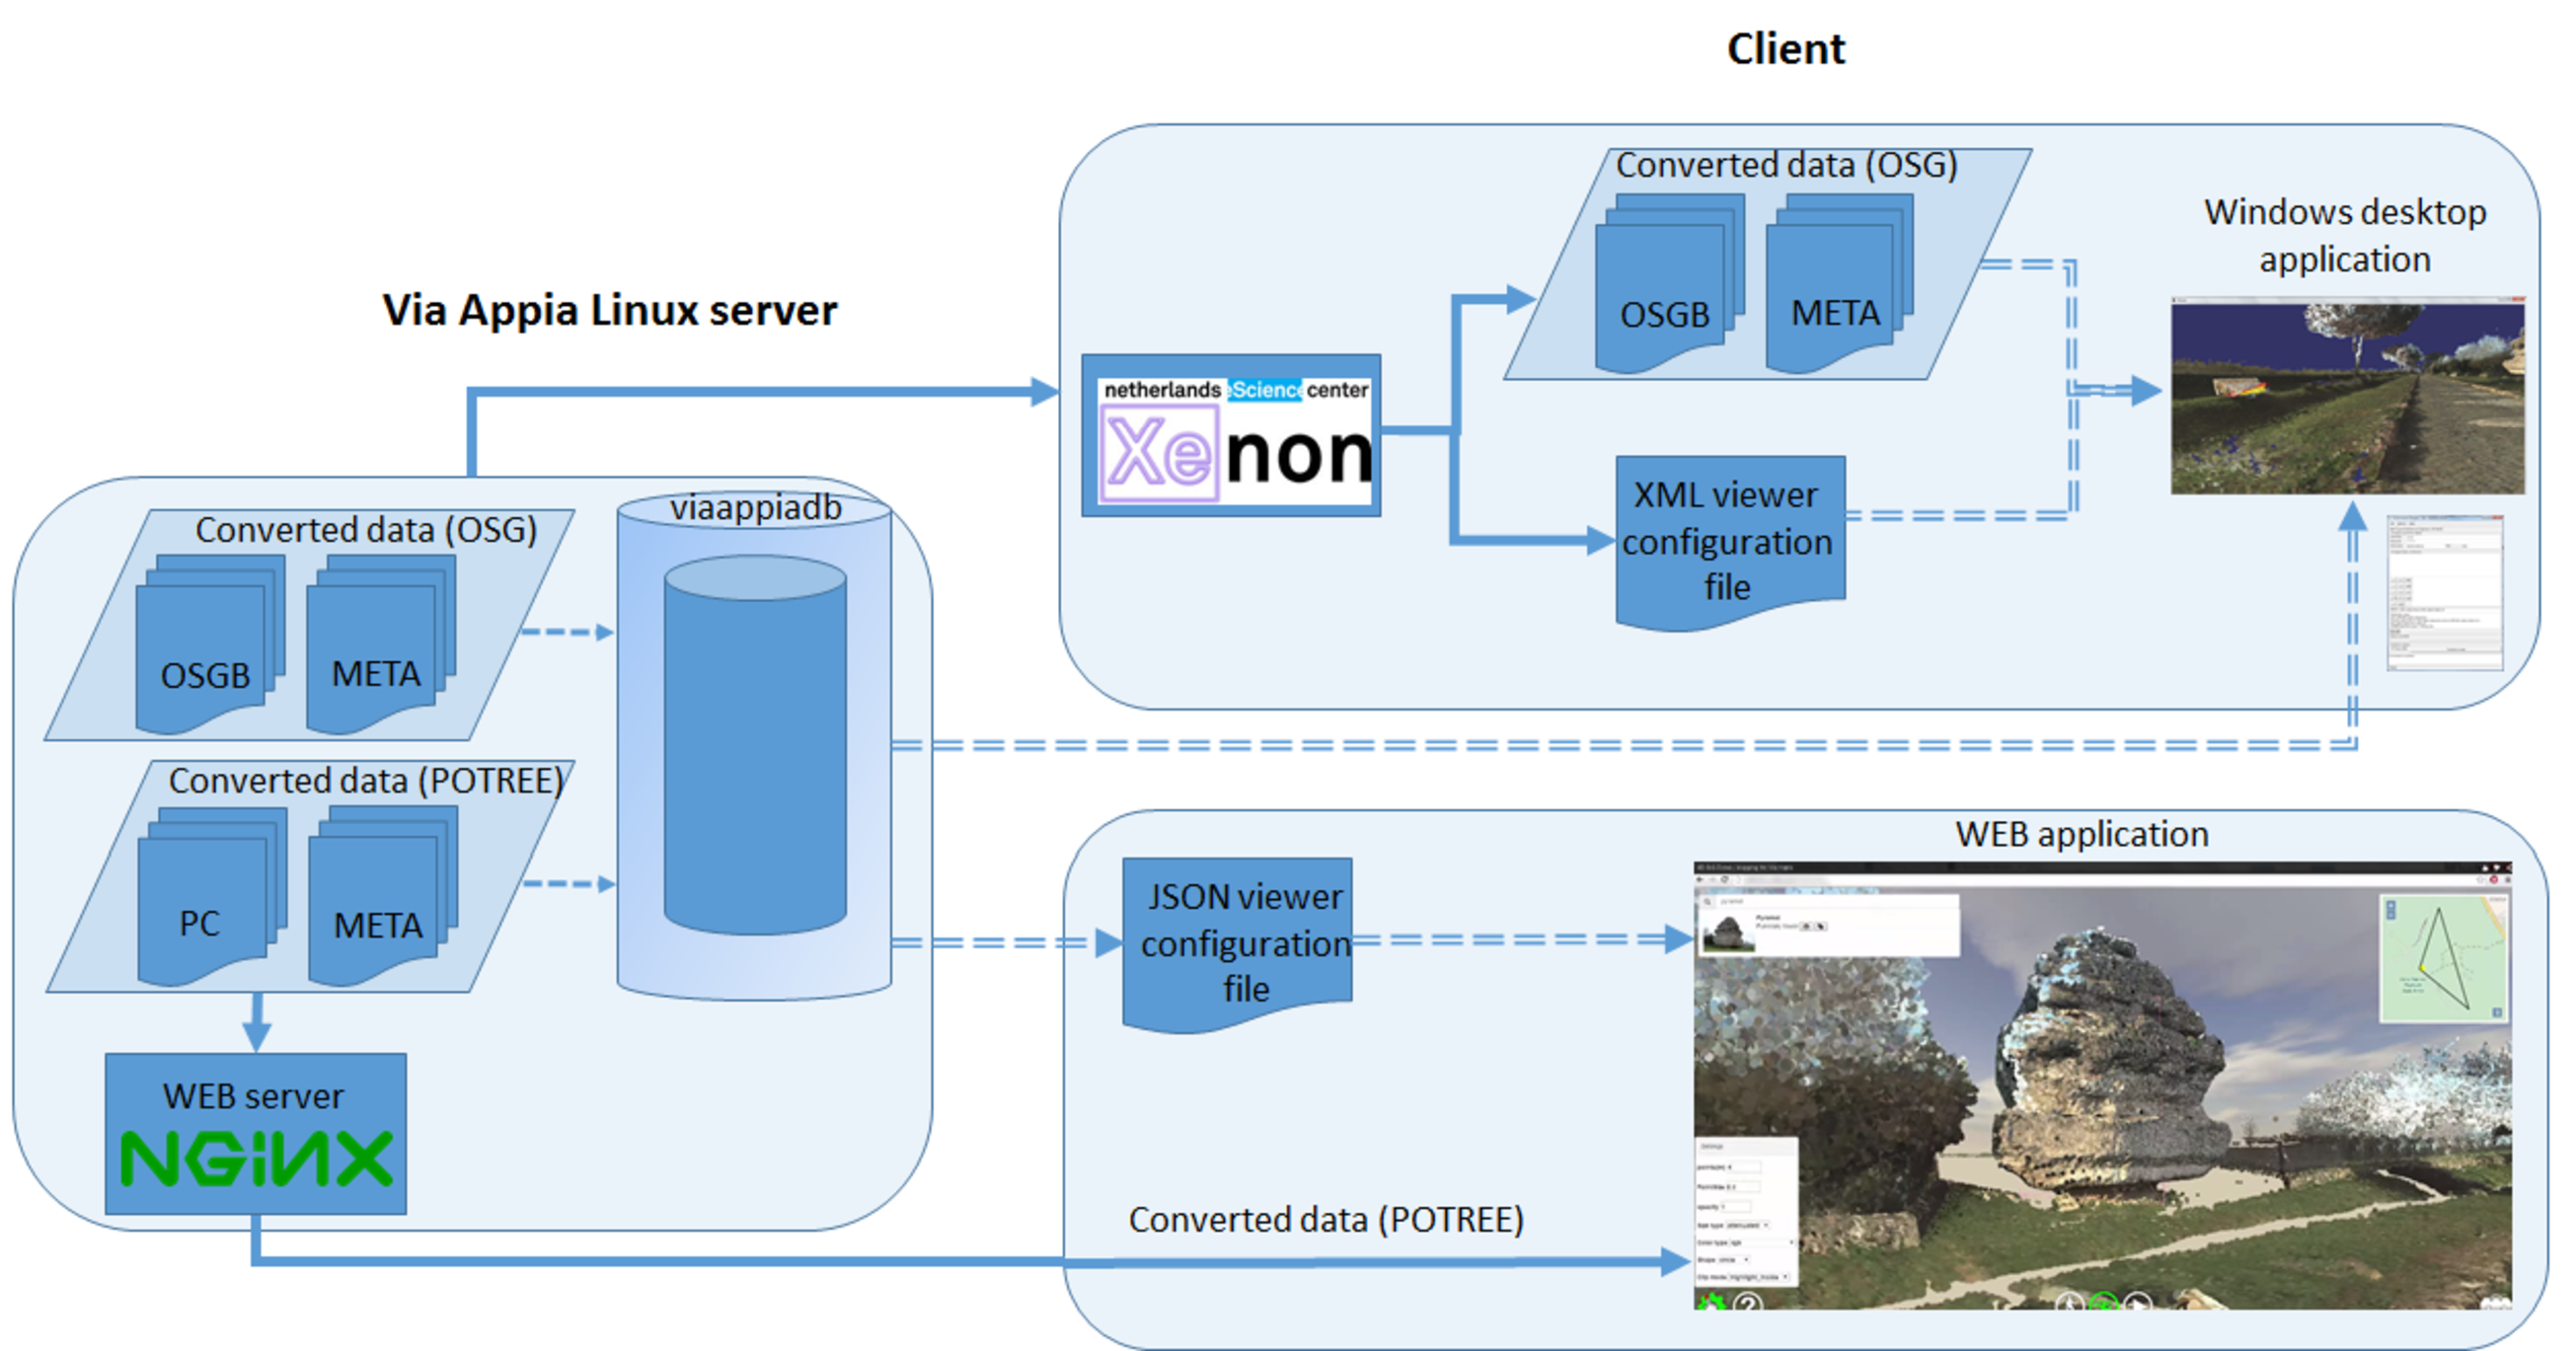
\includegraphics[width=0.4\textwidth]{fig/system_architecture/TwoTierArchitecture.pdf}
 \caption{}
 \label{fig:sys_arch_2tier}
\end{figure}